\section{Embedding Method: Word2Vec}
\begin{frame}{}
    \LARGE Embedding Method: \textbf{Word2Vec}
\end{frame}

\begin{frame}{Word Embeddings – Intuition}
    \begin{itemize}
        \item Dense vector representations of words learned from context.
        \item Encode syntactic and semantic meaning.
        \item Vectors reflect relationships like synonymy, analogy, etc.
    \end{itemize}
\end{frame}

\begin{frame}{Basic Word Embedding Methods}
    \begin{itemize}
        \item \textbf{word2vec} (Google, 2013)
        \begin{itemize}
            \item Continuous bag-of-words (CBOW)
            \item Continuous skip-gram / Skip-gram with negative sampling (SGNS)
        \end{itemize}
        \item \textbf{Global Vectors (GloVe)} (Stanford, 2014)
        \item \textbf{fastText} (Facebook, 2016)
        \begin{itemize}
            \item Supports out-of-vocabulary (OOV) words
        \end{itemize}
    \end{itemize}
\end{frame}

\begin{frame}{Advanced Word Embedding Methods}
    \begin{itemize}
        \item Deep learning-based, contextual embeddings:
        \begin{itemize}
            \item \textbf{BERT} (Google, 2018)
            \item \textbf{ELMo} (Allen Institute for AI, 2018)
            \item \textbf{GPT-2} (OpenAI, 2018)
        \end{itemize}
        \item Tunable pre-trained models available
    \end{itemize}
\end{frame}

\begin{frame}{Word2Vec Overview}
    \begin{itemize}
        \item Word2Vec learns word embeddings from large text corpora.
        \item Two main architectures:
        \begin{itemize}
            \item Continuous Bag-of-Words (CBOW)
            \item Skip-gram
        \end{itemize}
        \item Both models use neural networks to predict words based on context.
    \end{itemize}
\end{frame}

\subsection{Word2Vec – Continuous Bag-of-Words (CBOW)}
\begin{frame}[allowframebreaks]{Word2Vec – CBOW}
    \begin{itemize}
        \item \textbf{Goal:} Predict target word from context.
        \item \textbf{Architecture:}
        \begin{itemize}
            \item \textbf{Input:} Surrounding words (context)
            \item \textbf{Output:} Target word
        \end{itemize}
        \item Fast and accurate for frequent words.
        \item \textbf{Example:}
        \begin{itemize}
            \item Context: ``the \_\_\_ sat on the mat'' $\rightarrow$ Predict ``cat''
        \end{itemize}
    \end{itemize}
\framebreak
    \begin{figure}
        \centering
        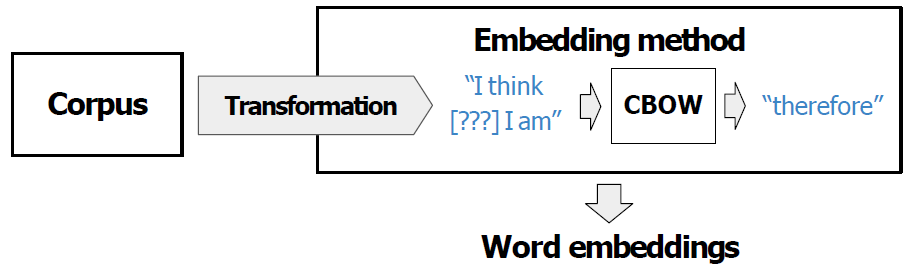
\includegraphics[width=\textwidth,height=0.8\textheight,keepaspectratio]{images/vector-space/cbow-1.png}
        \caption{CBOW Architecture}
    \end{figure}
\end{frame}

\begin{frame}[allowframebreaks]{Center word prediction: rationale}
    \begin{figure}
        \centering
        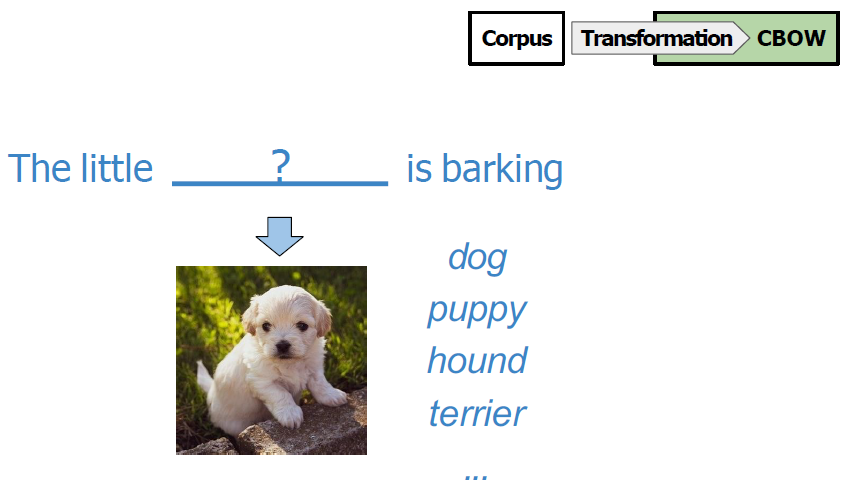
\includegraphics[width=\textwidth,height=0.8\textheight,keepaspectratio]{images/vector-space/center-word-pred.png}
    \end{figure}
\end{frame}

\begin{frame}[allowframebreaks]{Creating a training example}
    \begin{figure}
        \centering
        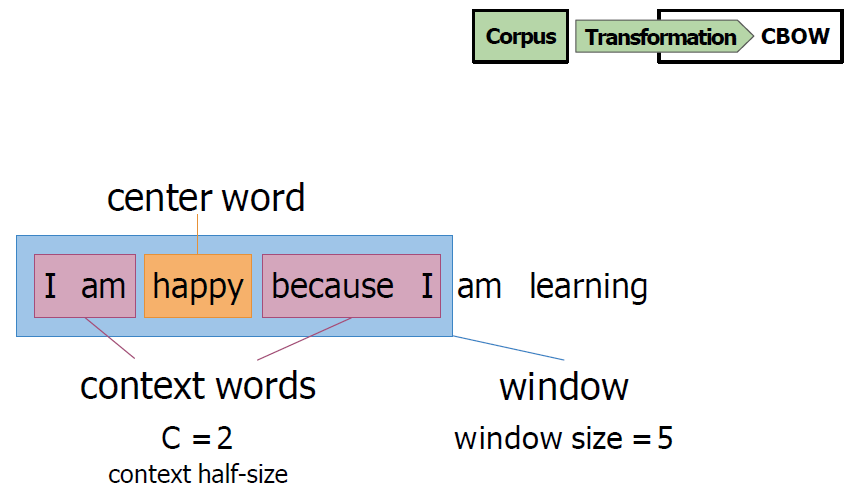
\includegraphics[width=\textwidth,height=0.8\textheight,keepaspectratio]{images/vector-space/training-example.png}
    \end{figure}
\end{frame}

\begin{frame}[allowframebreaks]{From corpus to training}
    \begin{figure}
        \centering
        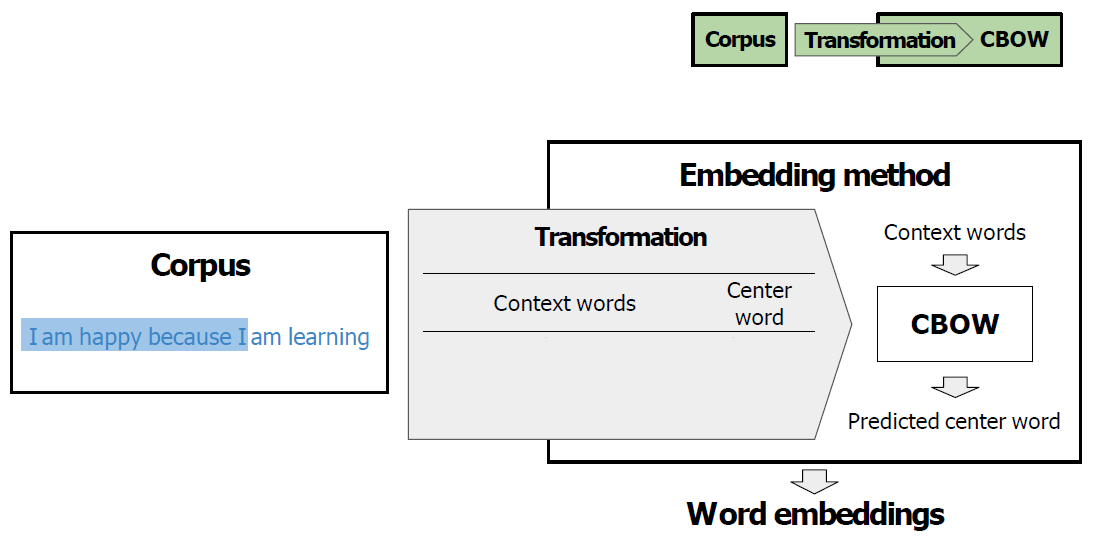
\includegraphics[width=\textwidth,height=0.8\textheight,keepaspectratio]{images/vector-space/corpus2training.png}
    \end{figure}
\end{frame}

\subsection{Word2Vec – Skip-Gram}
\begin{frame}[allowframebreaks]{Word2Vec – Skip-Gram}
    \begin{itemize}
        \item \textbf{Goal:} Predict context words from a target word.
        \item \textbf{Architecture:}
        \begin{itemize}
            \item \textbf{Input:} Target word
            \item \textbf{Output:} Surrounding words (context)
        \end{itemize}
        \item Better for rare words.
        \item \textbf{Example:}
        \begin{itemize}
            \item Input: ``cat'' $\rightarrow$ Output: ``the'', ``sat'', ``on'', ``the'', ``mat''
        \end{itemize}
    \end{itemize}
\framebreak
    \begin{figure}
        \centering
        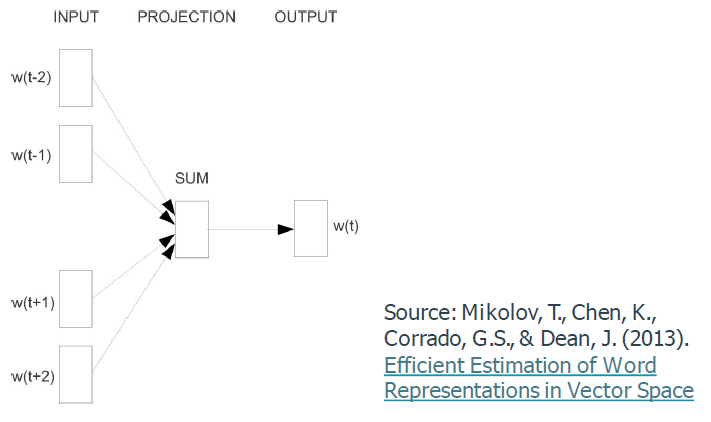
\includegraphics[width=\textwidth,height=0.8\textheight,keepaspectratio]{images/vector-space/skipgram-1.png}
        \caption{Skip-Gram Architecture}
    \end{figure}
\framebreak
    \begin{figure}
        \centering
        \fetchconvertimage{https://miro.medium.com/v2/resize:fit:1400/0*yxs3JKs5bKc4c_i8.png}{images/vector-space/skipgram-2.png}{width=\textwidth,height=0.9\textheight,keepaspectratio}
    \end{figure}
\end{frame}

\begin{frame}[allowframebreaks]{CBOW vs Skip-Gram}
    \begin{figure}
        \centering
        \fetchconvertimage{https://miro.medium.com/v2/resize:fit:1200/1*xC6wfTU_zpUlpRlXs5NZ4w.png}{images/vector-space/cbow-skipgram.png}{width=\textwidth,height=0.9\textheight,keepaspectratio}
    \end{figure}
\end{frame}

\begin{frame}{Limitations of Word2Vec}
    \begin{itemize}
        \item Does not consider sub-word information.
        \item Same vector for all senses of a word (polysemy issue).
        \item Ignores word order within the context window.
    \end{itemize}
\end{frame}